\documentclass{beamer}
\usetheme{Boadilla}
% \renewcommand{\baselinestretch}{1.5}

\usepackage{physics} % better derivative writings
\usepackage{unicode-math}

\NewDocumentCommand{\e}{}{\symrm{e}}

\title{Maclaurin Series}
\author{Kutay}
\institute{Made with LaTeX}
\date{\today}

% \parskip=10pt

% \setkomafont{disposition}{\normalfont\bfseries}

\begin{document}

\begin{frame}
  \titlepage
\end{frame}

\begin{frame}
  \frametitle{Outline}
  \tableofcontents
\end{frame}

\section{What is it?}

\begin{frame}
  \frametitle{What is it?}
  \begin{itemize}
    \item Approximation of a function with an infinite series
    \item Approximates near 0
  \end{itemize}
\end{frame}

\section{Why?}

\begin{frame}
  \frametitle{Why?}
  \begin{itemize}
    \item To compute \( \sin x \), \( \cos x \), and \( \e^x \) \textit{fast}
    \item Calculators (your TI) use this technique
    \item To simplify equations/functions
    \item In simple pendulum, we \textit{approximated} \( \sin x \) with \( x \)
  \end{itemize}
\end{frame}

\section{Derivation}

\begin{frame}
  \frametitle{Derivation}
  \begin{itemize}
    \item Calculators can multiply, add, subtract, divide, and take powers of whole numbers \textit{quickly}
    \item Let us use \textit{polynomials}
    \item Polynomials are just multiplications, additions, and exponentiations
  \end{itemize}
\end{frame}

\begin{frame}
  \frametitle{Derivation}
  \begin{figure}[ht]
    \centering
    \caption{The Function \( \cos x \)}
    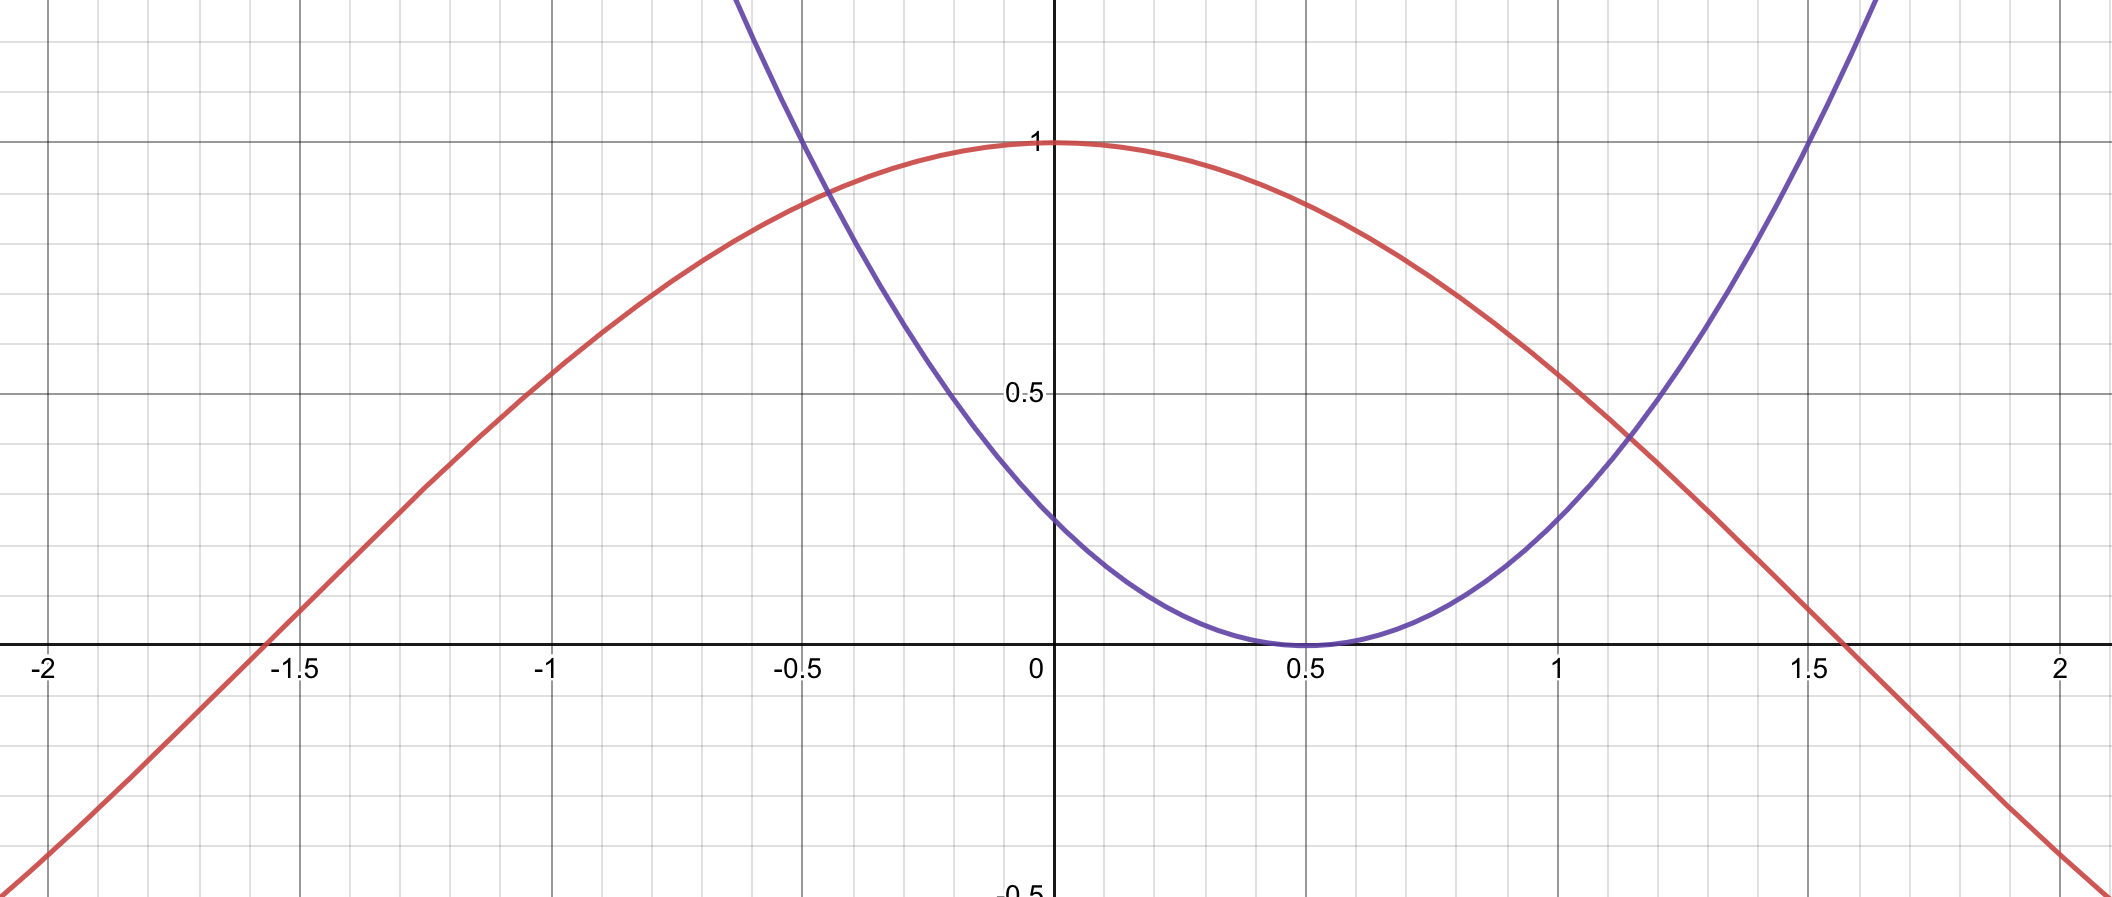
\includegraphics[
      scale=0.13
    ]{images/cosx.png}
  \end{figure}
  \begin{itemize}
    \item Approximate to two degrees
    \item Find real numbers for \( a, b, \) and \( c \) that approximate \( \cos x \) the \textit{best}
  \end{itemize}
  \begin{equation*}
    \cos x \approx a + bx + cx^2
  \end{equation*}
\end{frame}

\begin{frame}
  \frametitle{Derivation}
  \begin{itemize}
    \item We want to approximate \textit{near} \( x = 0 \)
    \item \( \cos x = a + bx + cx^2 \) at \( x = 0 \)
  \end{itemize}
  \begin{align*}
    \cos 0 &= a + b \cdot 0 + c \cdot 0^2 \\
    1 &= a
  \end{align*}
  \begin{figure}[ht]
    \centering
    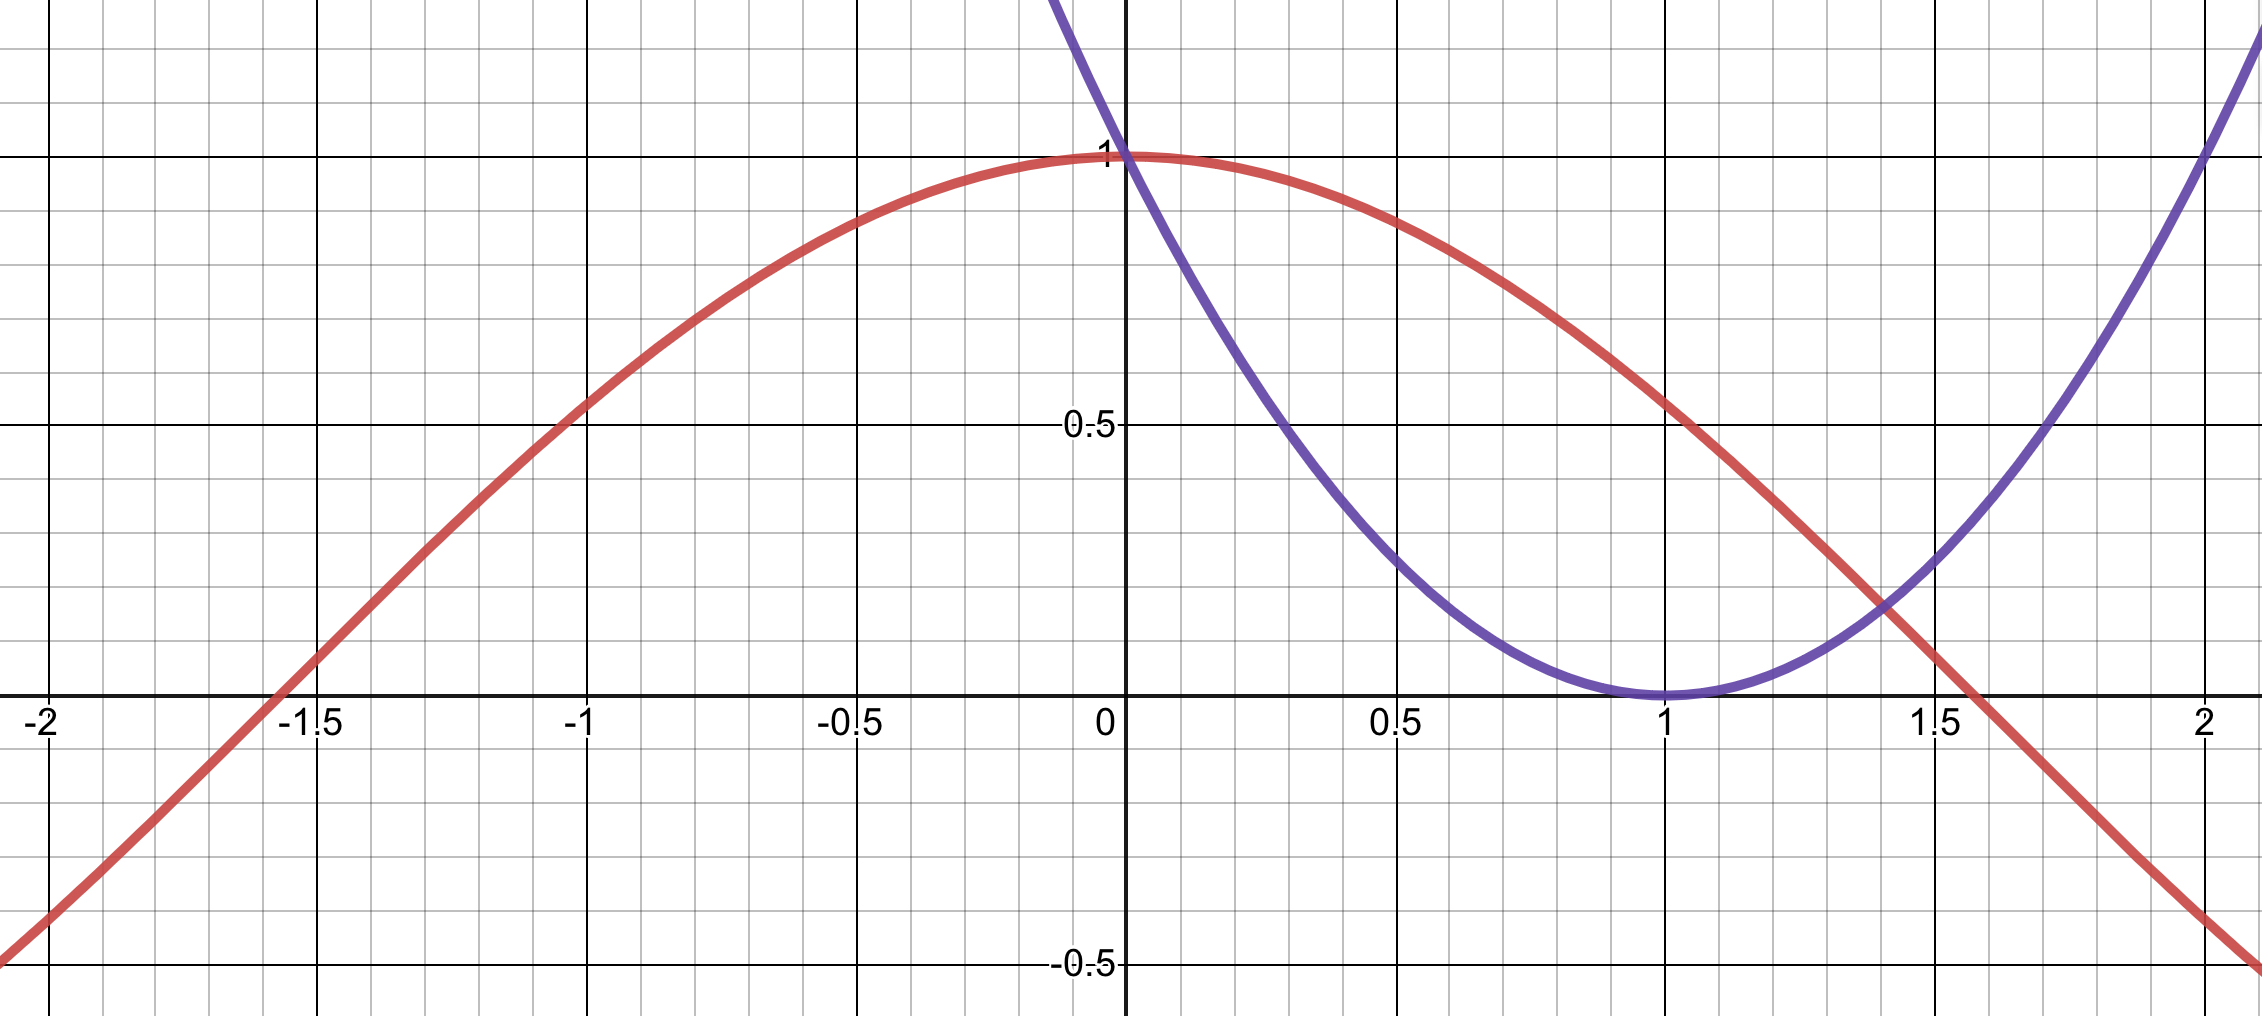
\includegraphics[
      scale=0.14
    ]{images/first.png}
  \end{figure}
\end{frame}

\begin{frame}
  \frametitle{Derivation}
  \begin{figure}[ht]
    \centering
    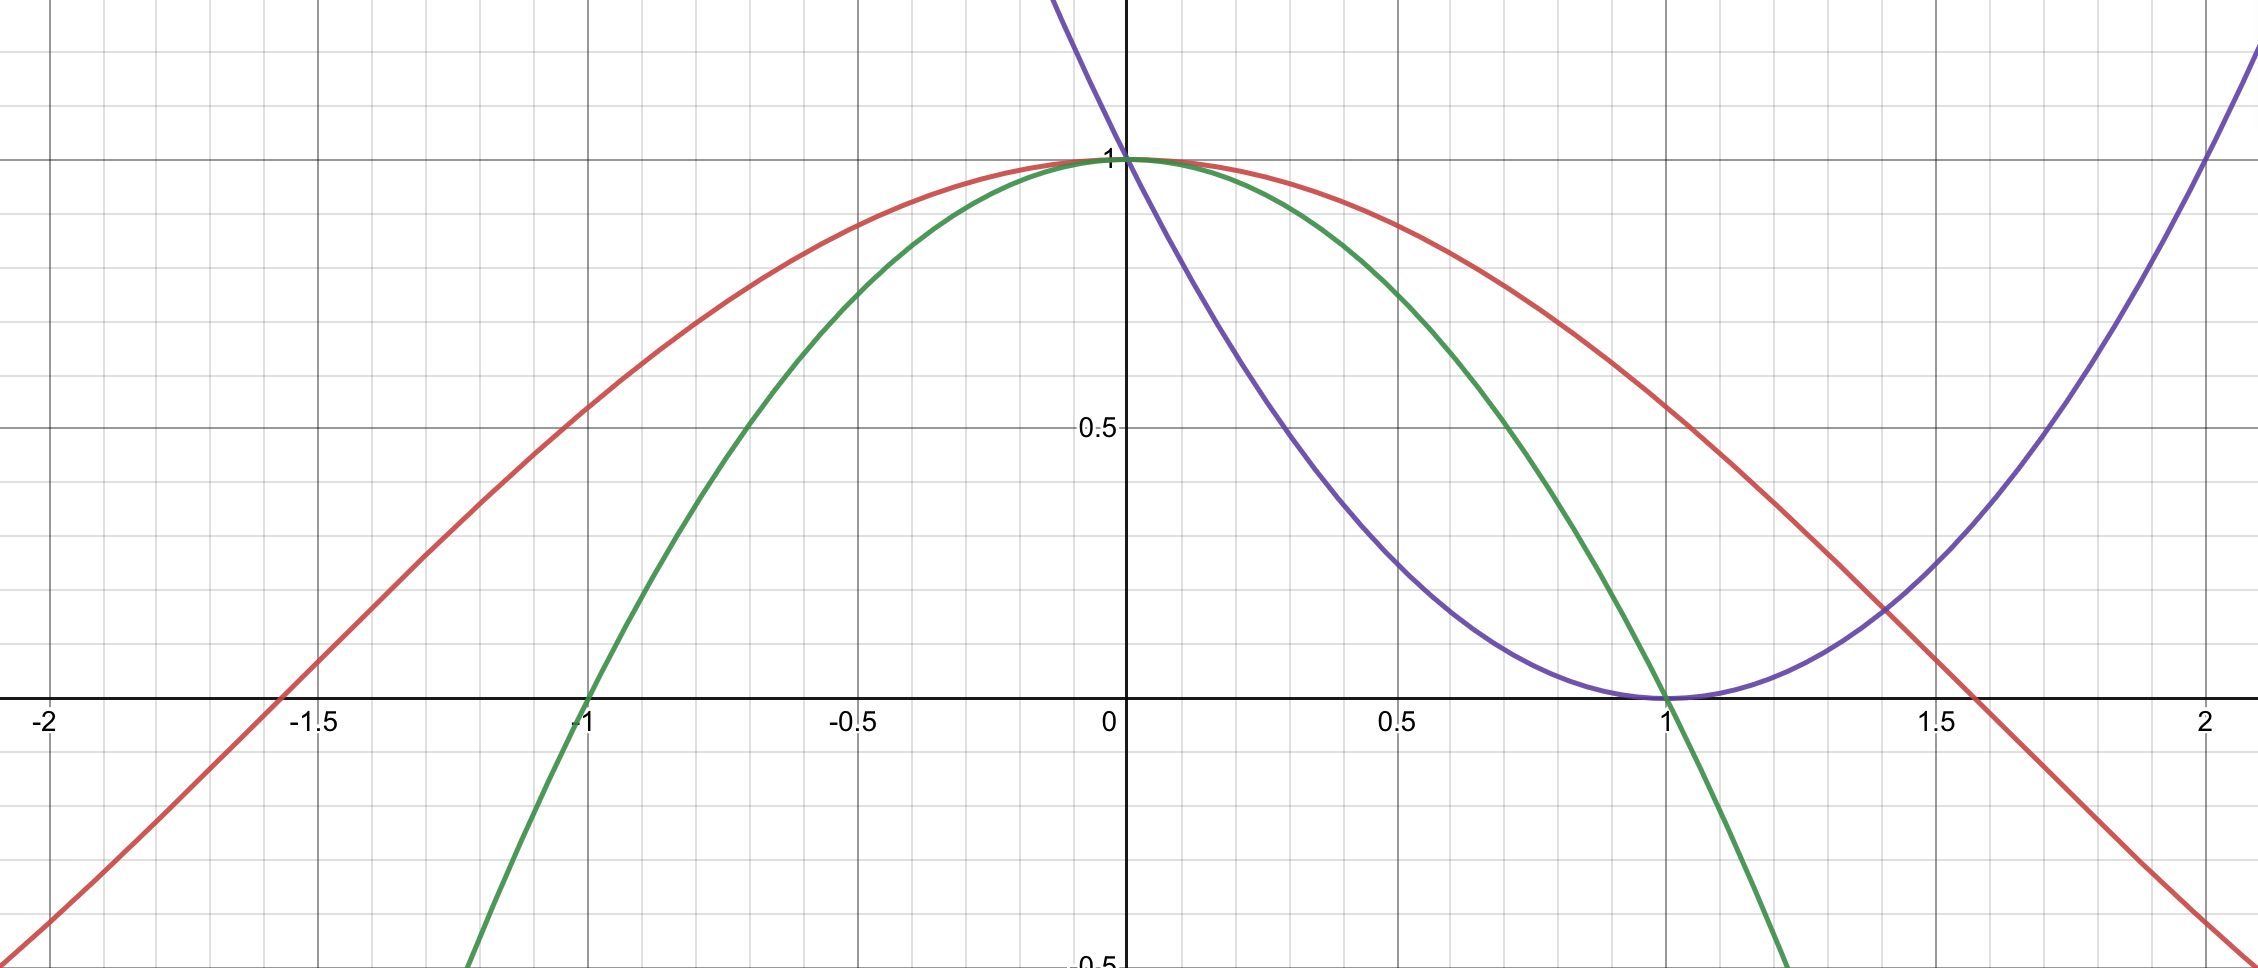
\includegraphics[
      scale=0.12
    ]{images/second.png}
  \end{figure}
  \begin{itemize}
    \item The green function is better, but why?
    \item The rate of change is the same as \( \cos x \) at \( x = 0 \)
    \item Our approximation must have the same derivative at \( x = 0 \)
    \item \( \cos' x = -\sin x \) and \( (a + bx + cx^2)' = b + 2cx \)
  \end{itemize}
  \begin{align*}
    -\sin 0 = 0 &= b + 2c \cdot 0 \\
    b &= 0
  \end{align*}
\end{frame}

\begin{frame}
  \frametitle{Derivation}
  \begin{figure}[ht]
    \centering
    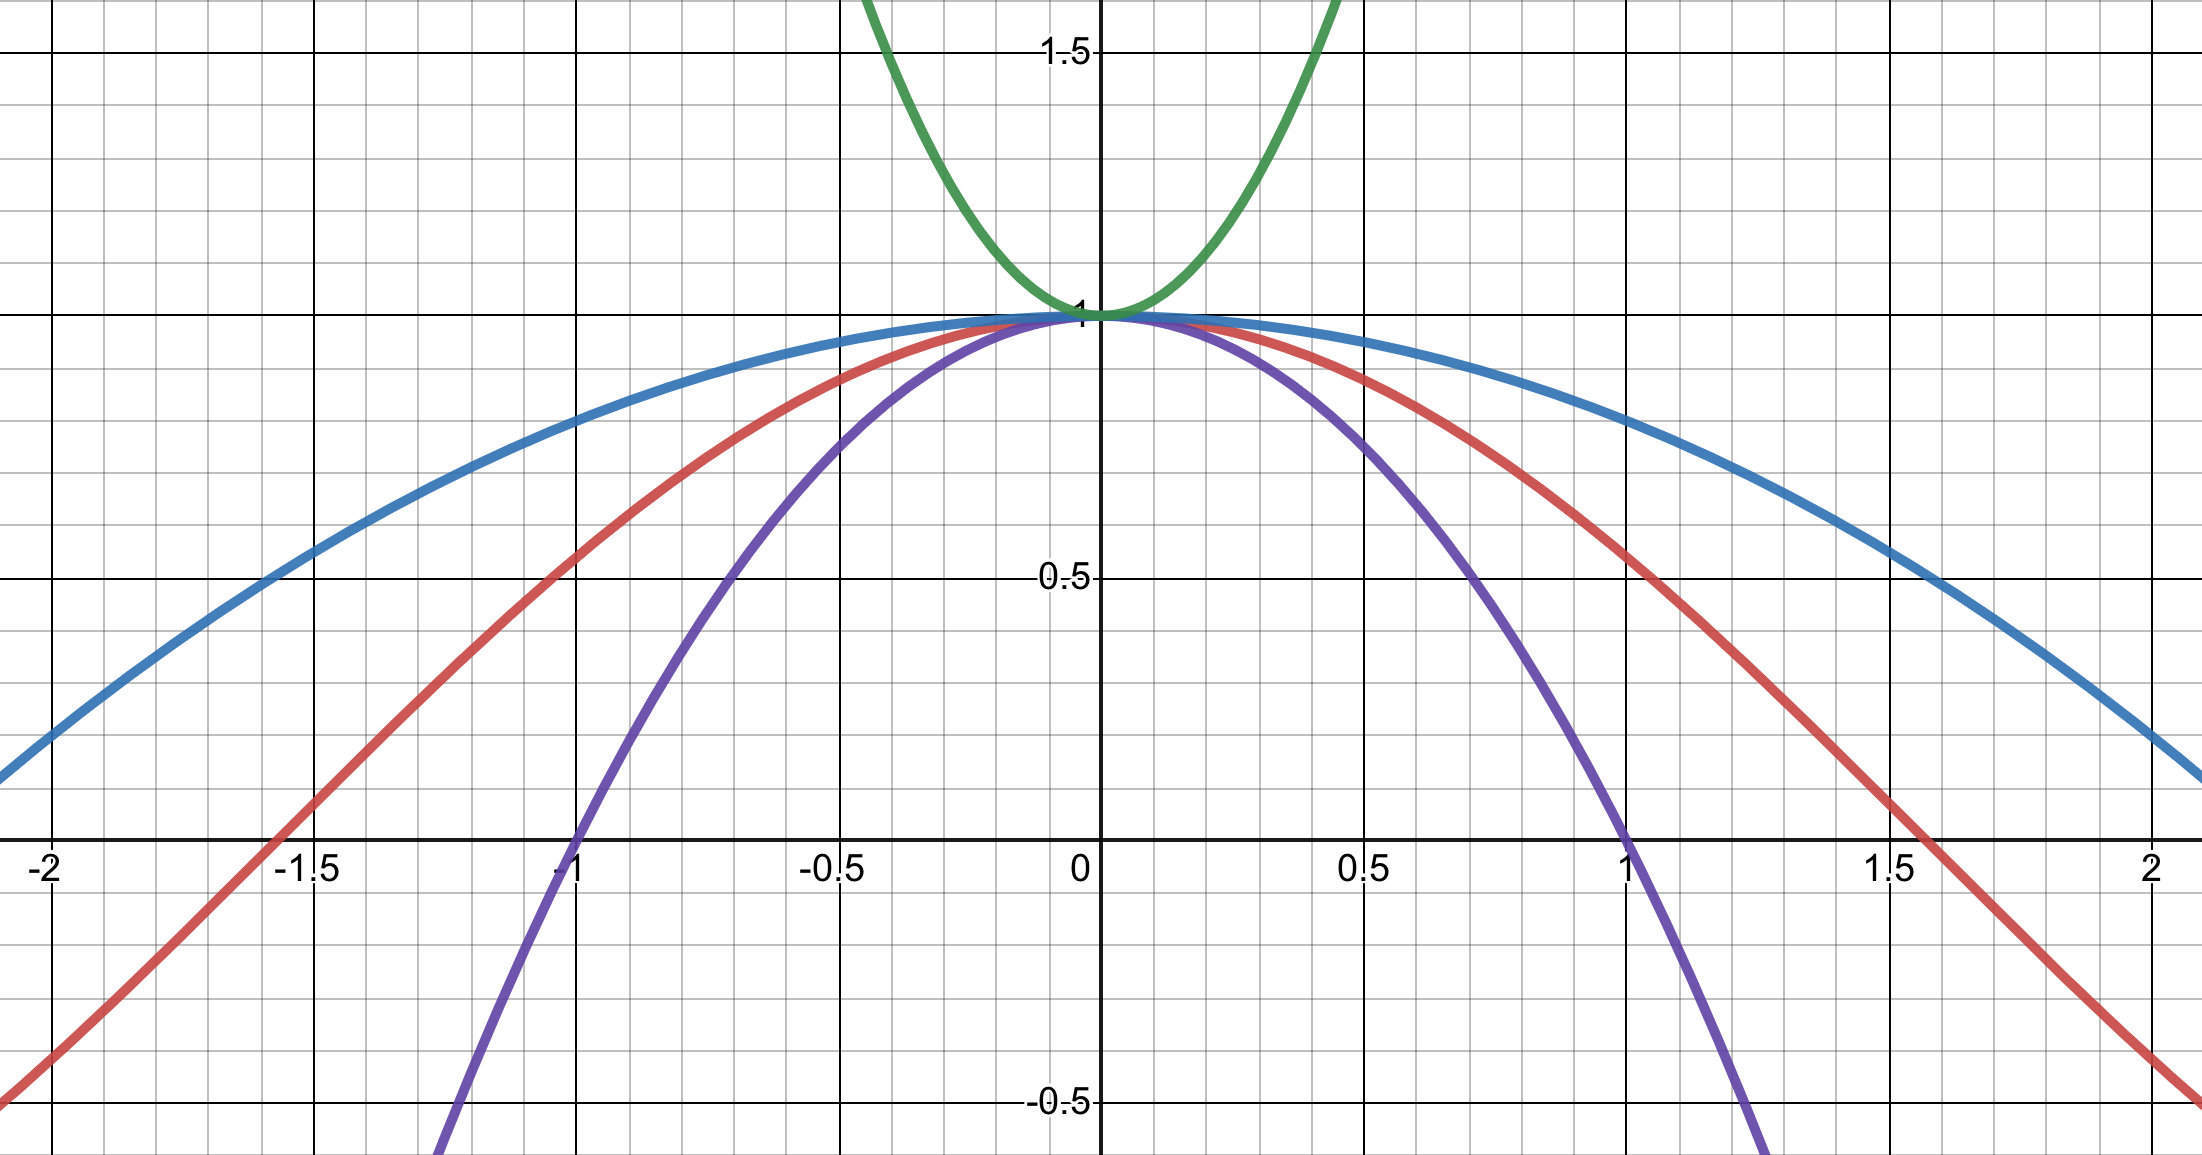
\includegraphics[
      scale=0.11
    ]{images/examples.png}
  \end{figure}
  \begin{itemize}
    \item \( \cos x \) \textit{curves} downwards at \( x = 0 \)
    \item So, the second derivative is negative
    \item Which means the rate of change is decreasing
    \item Same second derivative will ensure that they curve at the same rate
  \end{itemize}
  \begin{align*}
    \cos'' x &= -\cos x \\
    (a + bx + cx^2)'' &= 2c
  \end{align*}
\end{frame}

\end{document}
